% =====================================================================
%  Slide bài tập lớn Khai phá dữ liệu – Thuật toán K-Nearest Neighbors
%  Phong cách theo bài giảng của học phần (nền trắng, tam giác xanh)
%  Biên dịch bằng XeLaTeX (Overleaf: Menu -> Compiler -> XeLaTeX)
% =====================================================================
\documentclass[aspectratio=169,10pt]{beamer}

\usepackage{fontspec}
% Font theo tên file: có sẵn trong TeX Live, MiKTeX và Overleaf
\setsansfont{texgyreheros}[Extension=.otf, UprightFont=*-regular, BoldFont=*-bold,
  ItalicFont=*-italic, BoldItalicFont=*-bolditalic]
\newfontfamily\titlefont{texgyreadventor}[Extension=.otf, UprightFont=*-regular, BoldFont=*-bold]
\usepackage{amsmath,amssymb}
\usepackage{booktabs,array,tabularx,colortbl}
\usepackage{graphicx}
\usepackage{tikz}
\usetikzlibrary{arrows.meta,positioning}
\graphicspath{{figures/}}

% ---------------------------------------------------------------- Màu
\definecolor{tieude}{HTML}{4BB8E5}   % xanh nhạt của tiêu đề
\definecolor{chu}{HTML}{3F3F3F}      % chữ xám đậm
\definecolor{nhan}{HTML}{E0312B}     % đỏ nhấn mạnh
\definecolor{xanh}{HTML}{1F77B4}
\definecolor{t1}{HTML}{D3EEFA}
\definecolor{t2}{HTML}{8FD3F2}
\definecolor{t3}{HTML}{55BCE9}
\definecolor{t4}{HTML}{2B8FCB}
\definecolor{t5}{HTML}{2A6A9C}
\definecolor{bang}{HTML}{E8F5FC}

\newcommand{\hl}[1]{\textcolor{nhan}{\textbf{#1}}}
\newcommand{\hx}[1]{\textcolor{xanh}{\textbf{#1}}}

% ---------------------------------------------------------------- Nền: các tam giác xanh
\setbeamertemplate{background}{%
  \begin{tikzpicture}[remember picture,overlay]
    \begin{scope}[shift={(current page.south west)}]
      % dải trái
      \fill[t2] (0,9) -- (0.85,9) -- (0,3.6) -- cycle;
      \fill[t3!70] (0,0) -- (0.45,0) -- (0,2.6) -- cycle;
      % cụm phải
      \fill[t1] (12.25,9) -- (13.2,9) -- (15.1,0) -- (11.9,0) -- cycle;
      \fill[t2] (12.7,9) -- (14.5,9) -- (15.7,0) -- (13.7,0) -- cycle;
      \fill[t3] (14.0,9) -- (16,9) -- (16,0) -- (14.6,0) -- cycle;
      \fill[t5] (14.75,9) -- (16,9) -- (16,2.6) -- cycle;
      \fill[t4] (12.6,0) -- (16,0) -- (16,3.8) -- cycle;
      \draw[t3, line width=0.3pt] (12.25,9) -- (14.85,0);
      \draw[t3, line width=0.3pt] (9.6,0) -- (16,3.9);
    \end{scope}
  \end{tikzpicture}}

\setbeamersize{text margin left=1.25cm, text margin right=3.6cm}
\setbeamertemplate{navigation symbols}{}
\setbeamercolor{normal text}{fg=chu}
\setbeamercolor{frametitle}{fg=tieude}
\setbeamerfont{frametitle}{size=\LARGE}
\setbeamertemplate{frametitle}{\vspace*{0.55cm}{\titlefont\insertframetitle}\par\vspace*{-0.1cm}}
\setbeamertemplate{footline}{\hspace*{1.25cm}{\fontsize{6}{7}\selectfont\color{gray}\insertframenumber}\vspace*{0.25cm}}

% Ký hiệu đầu dòng: tam giác xanh như bài giảng
\setbeamertemplate{itemize item}{\color{tieude}\raisebox{0.1ex}{\tikz\fill (0,0) -- (0.19,0.11) -- (0,0.22) -- cycle;}}
\setbeamertemplate{itemize subitem}{\color{tieude}\raisebox{0.1ex}{\tikz\fill (0,0) -- (0.15,0.085) -- (0,0.17) -- cycle;}}
\setbeamertemplate{enumerate item}{\color{tieude}\insertenumlabel.}
\setlength{\leftmargini}{1.4em}
\setbeamerfont{itemize/enumerate subbody}{size=\small}

% Hộp nền xanh rất nhạt (cho công thức, kết luận)
\newcommand{\hop}[1]{\begin{center}\colorbox{bang}{\parbox{0.92\linewidth}{\centering #1}}\end{center}}

% Slide mục lục: mục hiện tại phóng to
\newcommand{\mucluc}[1]{%
  \begin{frame}[plain]
    \vspace*{1.6cm}
    \begin{itemize}\setlength\itemsep{0.5em}
      \ifnum#1=1 \item {\Huge Giới thiệu}\else \item {\large Giới thiệu}\fi
      \ifnum#1=2 \item {\Huge Công việc liên quan}\else \item {\large Một số công việc liên quan}\fi
      \ifnum#1=3 \item {\Huge Thuật toán KNN}\else \item {\large Thuật toán KNN}\fi
      \ifnum#1=4 \item {\Huge Thực nghiệm}\else \item {\large Thực nghiệm và phân tích kết quả}\fi
      \ifnum#1=5 \item {\Huge Kết luận}\else \item {\large Kết luận}\fi
    \end{itemize}
  \end{frame}}

% ---------------------------------------------------------------- Thông tin nhóm (TODO: điền)
\newcommand{\gvhd}{TS. Trịnh Thành}
\newcommand{\thanhvien}{Nguyễn Tuấn Anh (23010575) \quad Lê Anh Duy (23010710) \quad Đinh Xuân Tài (23010616)}

\begin{document}

% =====================================================================
% TRANG BÌA
% =====================================================================
\begin{frame}[plain]
  \begin{tikzpicture}[remember picture,overlay]
    \node[anchor=east, align=right, text width=10cm] at ([xshift=-4.1cm,yshift=0.3cm]current page.east)
      {{\titlefont\color{tieude}\fontsize{30}{34}\selectfont K-Nearest\\[2pt] Neighbors (KNN)}\\[10pt]
       {\large\color{gray} Thuật toán K láng giềng gần nhất}\\[2pt]
       {\normalsize\color{gray} và ứng dụng phân loại hoa Iris}\\[14pt]
       {\small\color{gray} Học phần: Khai phá dữ liệu}\\[2pt]
       {\small\color{gray} Giảng viên hướng dẫn: \gvhd}\\[6pt]
       {\footnotesize\color{gray} Nguyễn Tuấn Anh -- 23010575}\\
       {\footnotesize\color{gray} Lê Anh Duy -- 23010710}\\
       {\footnotesize\color{gray} Đinh Xuân Tài -- 23010616}};
  \end{tikzpicture}
\end{frame}

\mucluc{0}

% =====================================================================
% 1. GIỚI THIỆU
% =====================================================================
\mucluc{1}

\begin{frame}{Đặt vấn đề}
\begin{columns}[c,totalwidth=\textwidth]
\begin{column}{0.56\textwidth}
\begin{itemize}\setlength\itemsep{0.6em}
  \item Bài toán: xác định loài của một bông hoa Iris mới -- \hl{Setosa}, \hl{Versicolor} hay \hl{Virginica}
  \item Cách tiếp cận của nhà thực vật học:
  \begin{itemize}
    \item Đối chiếu với các mẫu đã biết loài có kích thước \textbf{tương đồng nhất}
    \item Xem xét loài của các mẫu tương đồng đó
    \item Kết luận theo \textbf{đa số}
  \end{itemize}
  \item Hình thức hóa quá trình này thành thuật toán $\Rightarrow$ \hx{KNN}
\end{itemize}
\end{column}
\begin{column}{0.4\textwidth}
\centering
\begin{tikzpicture}[font=\small]
  \foreach \i/\c in {0/red,1/red,2/xanh} \node[draw=gray,fill=white,minimum width=1.3cm,minimum height=0.8cm] (h\i) at (0,-\i*1.0) {\textcolor{\c}{Mẫu \the\numexpr\i+1\relax}};
  \node[draw=tieude,very thick,minimum width=1.4cm,minimum height=0.9cm] (m) at (2.6,-1) {\textbf{Hoa mới ?}};
  \foreach \i in {0,1,2} \draw[-{Stealth},gray] (m.west) -- (h\i.east);
  \node[align=center,font=\scriptsize] at (1.3,-2.9) {đối chiếu với các mẫu\\tương đồng nhất};
\end{tikzpicture}
\end{column}
\end{columns}
\end{frame}

\begin{frame}{Học máy và bài toán phân lớp}
\begin{itemize}\setlength\itemsep{0.7em}
  \item \textbf{Học máy (Machine Learning)}: máy tính tự rút ra quy luật từ dữ liệu, thay vì được lập trình sẵn từng quy tắc.
  \item \textbf{Phân lớp (classification)}:
  \begin{itemize}
    \item Cho các mẫu \textbf{đã biết nhãn} (dữ liệu huấn luyện)
    \item Xây dựng mô hình để \textbf{dự đoán nhãn cho mẫu mới}
    \item Ví dụ: phân loại thư rác; chẩn đoán khối u lành tính / ác tính
  \end{itemize}
  \item Các thuật toán phân lớp: Cây quyết định, Naive Bayes, SVM, Hồi quy Logistic, \hx{KNN}\ldots
  \item KNN là thuật toán \textbf{đơn giản và trực quan nhất}.
\end{itemize}
\end{frame}

\begin{frame}{KNN là gì?}
\begin{columns}[c,totalwidth=\textwidth]
\begin{column}{0.5\textwidth}
\begin{itemize}\setlength\itemsep{0.55em}
  \item KNN = \textbf{K láng giềng gần nhất}
  \item Giả định \hl{tương đồng cục bộ}: các điểm gần nhau có xu hướng cùng nhãn
  \item Dự đoán nhãn của điểm mới:
  \begin{itemize}
    \item Xác định \textbf{K láng giềng gần nhất}
    \item Thực hiện \textbf{biểu quyết đa số}
    \item Lớp có nhiều phiếu nhất là nhãn dự đoán
  \end{itemize}
  \item Không xây dựng mô hình tường minh, chỉ lưu trữ dữ liệu
  \item Thực nghiệm: phân loại hoa Iris (Fisher, 1936)
\end{itemize}
\end{column}
\begin{column}{0.48\textwidth}
  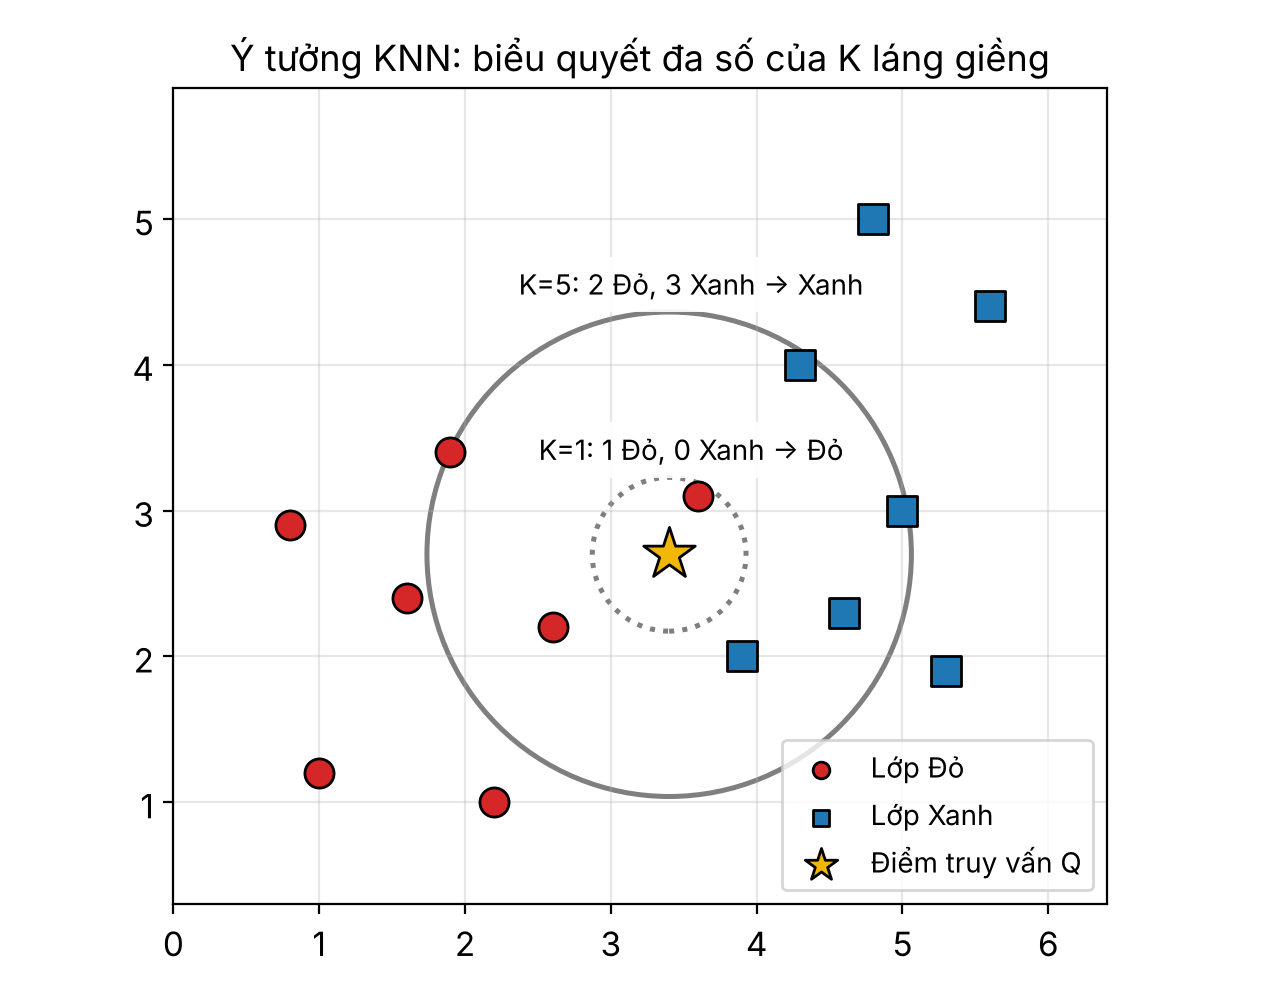
\includegraphics[width=\linewidth]{h0_y_tuong.png}
\end{column}
\end{columns}
\end{frame}

% =====================================================================
% 2. CÔNG VIỆC LIÊN QUAN
% =====================================================================
\mucluc{2}

\begin{frame}{Một số ứng dụng của KNN}
\begin{itemize}\setlength\itemsep{0.7em}
  \item \textbf{Y tế}: hỗ trợ chẩn đoán dựa trên các ca bệnh tương đồng
  \item \textbf{Hệ thống khuyến nghị}: lọc cộng tác theo người dùng / sản phẩm tương đồng
  \item \textbf{Nhận dạng mẫu}: chữ viết tay, hình ảnh
  \item \textbf{Điền giá trị khuyết thiếu}: ước lượng từ K mẫu tương đồng (KNN Imputation)
  \item \textbf{Truy vấn tương đồng}: tìm kiếm văn bản, hình ảnh theo biểu diễn vector
\end{itemize}
\end{frame}

\begin{frame}{Các công trình nghiên cứu liên quan}
\small
\renewcommand{\arraystretch}{1.35}
\begin{tabularx}{\linewidth}{@{}l l X@{}}
\rowcolor{bang}\textbf{Năm} & \textbf{Tác giả} & \textbf{Đóng góp chính}\\
1951 & Fix \& Hodges & Phân lớp phi tham số dựa trên láng giềng gần -- tiền thân của KNN\\
1967 & Cover \& Hart & Sai số tiệm cận của 1-NN $\le$ \hl{2 lần} sai số Bayes\\
1976 & Dudani & KNN có trọng số theo khoảng cách\\
1977 & Friedman và cs. & Cấu trúc KD-Tree tăng tốc truy vấn láng giềng\\
1999 & Beyer và cs. & Phân tích hiện tượng “lời nguyền số chiều”\\
2008 & Wu và cs. & KNN thuộc \hx{Top 10 thuật toán khai phá dữ liệu}\\
\end{tabularx}
\end{frame}

% =====================================================================
% 3. THUẬT TOÁN KNN
% =====================================================================
\mucluc{3}

\begin{frame}{Ý tưởng và bản chất}
\begin{itemize}\setlength\itemsep{0.6em}
  \item Giả định \hl{tương đồng cục bộ}: các điểm gần nhau trong không gian đặc trưng có xu hướng cùng nhãn
  \item Mỗi mẫu là một \textbf{điểm} trong không gian $d$ chiều, mỗi đặc trưng là một \textbf{trục tọa độ}
  \item Ba tính chất:
  \begin{itemize}\setlength\itemsep{0.3em}
    \item \textbf{Học lười (lazy learning)}: huấn luyện chỉ lưu trữ dữ liệu, chi phí tính toán dồn vào giai đoạn dự đoán
    \item \textbf{Phi tham số}: không giả định dạng hàm hay phân phối của dữ liệu
    \item \textbf{Dựa trên độ đo khoảng cách}: phụ thuộc độ đo và thang đo của đặc trưng
  \end{itemize}
\end{itemize}
\end{frame}

\begin{frame}{Cơ sở xác suất của biểu quyết}
\begin{itemize}\setlength\itemsep{0.6em}
  \item Tỉ lệ láng giềng thuộc lớp $c$ là ước lượng của \textbf{xác suất hậu nghiệm}:
\end{itemize}
\hop{$\displaystyle P(c \mid x) \approx \frac{k_c}{K}$ \qquad ($k_c$: số láng giềng thuộc lớp $c$, \ $K$: tổng số láng giềng)}
\begin{itemize}\setlength\itemsep{0.6em}
  \item Lớp có nhiều phiếu nhất $\equiv$ lớp có \textbf{xác suất hậu nghiệm lớn nhất}
  \item KNN xấp xỉ \hl{bộ phân lớp Bayes} -- bộ phân lớp có xác suất sai nhỏ nhất
  \item \textbf{Ví dụ} (thực nghiệm): $K = 19$, có 12 láng giềng Virginica
  \begin{itemize}
    \item $P(\text{Virginica}) \approx 12/19 = 0{,}63$ \quad $\Rightarrow$ dự đoán \hl{Virginica}
  \end{itemize}
\end{itemize}
\end{frame}

\begin{frame}{Ký hiệu và công thức}
\begin{columns}[T,totalwidth=\textwidth]
\begin{column}{0.42\textwidth}
\footnotesize
\renewcommand{\arraystretch}{1.25}
\begin{tabular}{@{}ll@{}}
\rowcolor{bang}\textbf{Ký hiệu} & \textbf{Ý nghĩa}\\
$n$ & số mẫu huấn luyện (120)\\
$d$ & số đặc trưng (2)\\
$x_i, y_i$ & đặc trưng, nhãn mẫu thứ $i$\\
$x$ & điểm truy vấn\\
$K$ & số láng giềng\\
$N_K(x)$ & K điểm gần $x$ nhất\\
$\hat y$ & nhãn dự đoán\\
\end{tabular}
\end{column}
\begin{column}{0.55\textwidth}
\textbf{Phân lớp} -- biểu quyết đa số:
\[\hat y = \arg\max_{c} \sum_{x_i \in N_K(x)} \mathbb{I}(y_i = c)\]
\vspace{0.2em}
{\small $\mathbb{I}(y_i = c) = 1$ nếu láng giềng thuộc lớp $c$, ngược lại $= 0$ \\ $\Rightarrow$ tổng $\Sigma$ = \textbf{số phiếu} của lớp $c$}

\vspace{0.6em}
\textbf{Hồi quy} -- lấy trung bình:
\[\hat y = \frac{1}{K}\sum_{x_i \in N_K(x)} y_i\]
\end{column}
\end{columns}
\end{frame}

\begin{frame}{Các bước của thuật toán}
\begin{itemize}
  \item Huấn luyện: \textbf{lưu trữ dữ liệu}. Với mỗi điểm truy vấn $x$, thực hiện 4 bước:
\end{itemize}
\vspace{0.2em}
\centering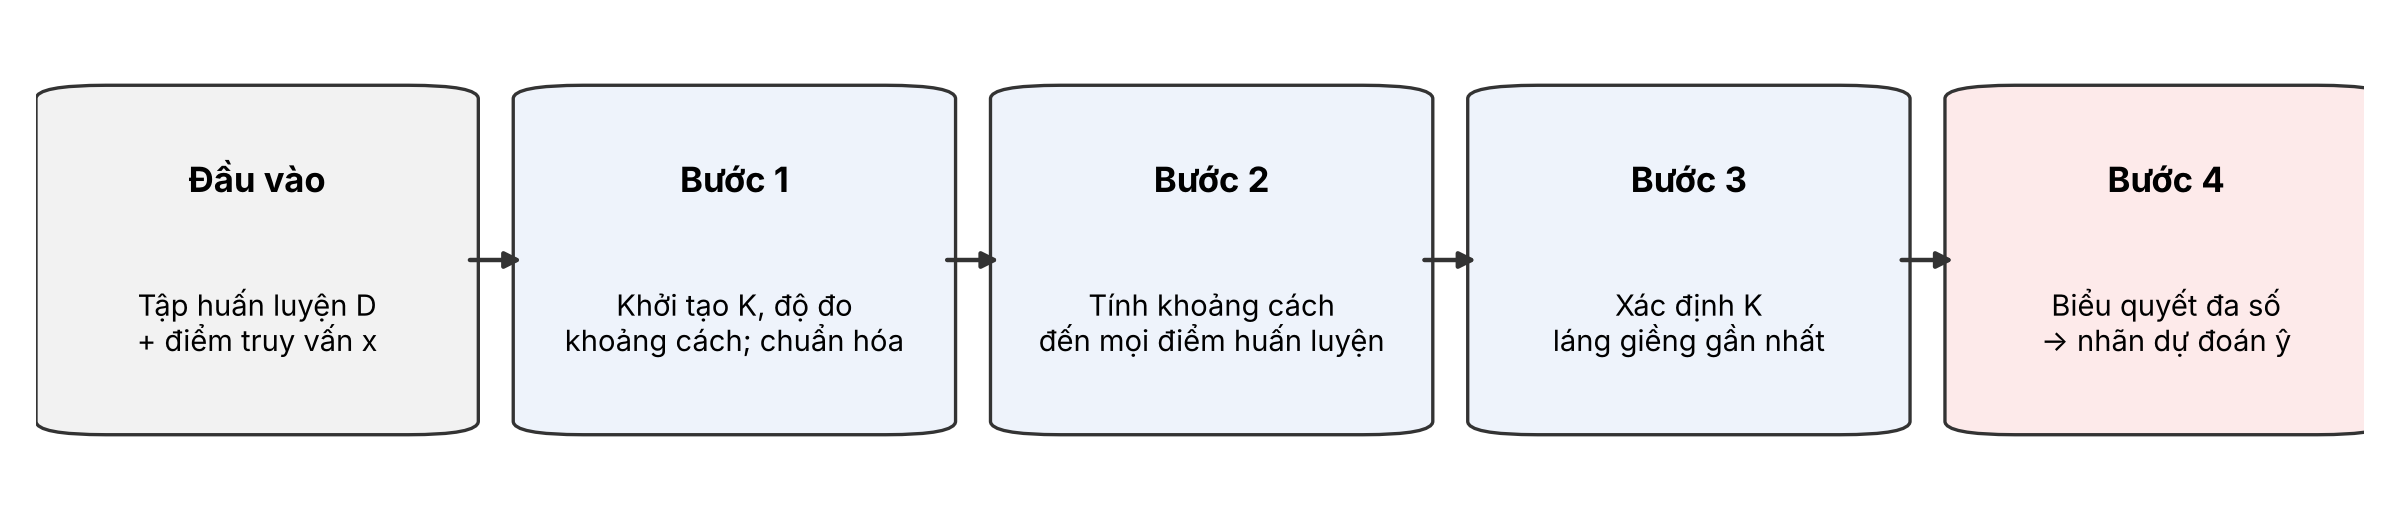
\includegraphics[width=\linewidth]{h7_so_do_khoi.png}
\hop{Khởi tạo tham số $\rightarrow$ Tính khoảng cách $\rightarrow$ Xác định K láng giềng $\rightarrow$ Biểu quyết đa số}
\end{frame}

\begin{frame}{Ví dụ minh họa}
\begin{columns}[c,totalwidth=\textwidth]
\begin{column}{0.47\textwidth}
\begin{itemize}\setlength\itemsep{0.5em}
  \item Tập huấn luyện gồm 6 điểm:
\end{itemize}
\small\centering
\renewcommand{\arraystretch}{1.2}
\begin{tabular}{ccc}
\rowcolor{bang}\textbf{Điểm} & \textbf{Tọa độ} & \textbf{Lớp}\\
A & (1; 1) & \textcolor{nhan}{Đỏ}\\
B & (2; 1) & \textcolor{nhan}{Đỏ}\\
C & (3; 1,5) & \textcolor{nhan}{Đỏ}\\
D & (4; 3) & \textcolor{xanh}{Xanh}\\
E & (5; 5) & \textcolor{xanh}{Xanh}\\
F & (6; 4) & \textcolor{xanh}{Xanh}\\
\end{tabular}
\begin{itemize}
  \item Phân lớp điểm truy vấn \hl{Q(3; 3)} với \hl{K = 3}
\end{itemize}
\end{column}
\begin{column}{0.5\textwidth}
  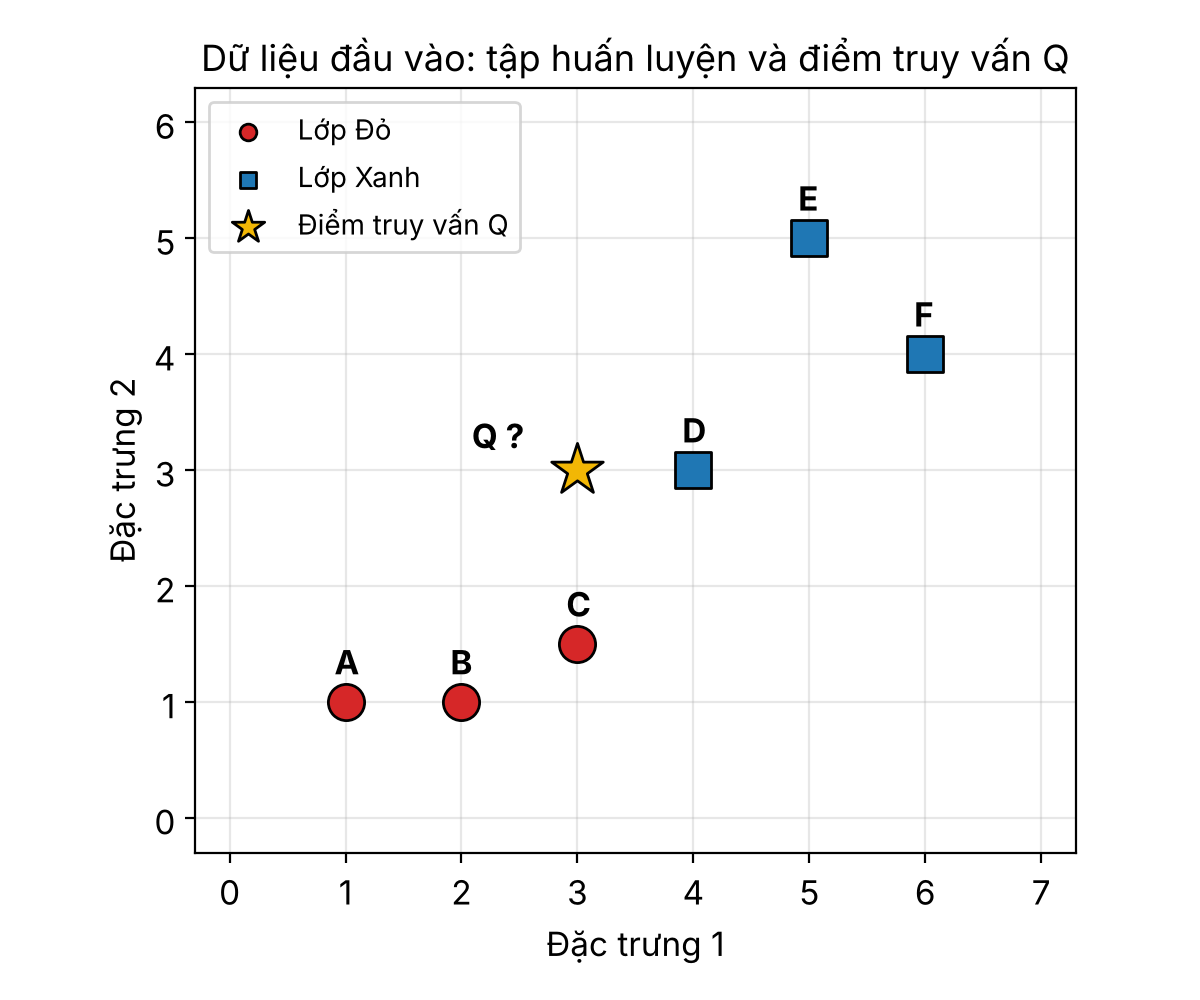
\includegraphics[width=\linewidth]{h1_dau_vao.png}
\end{column}
\end{columns}
\end{frame}

\begin{frame}{Bước 1 -- Khởi tạo và tiền xử lý}
\begin{itemize}\setlength\itemsep{0.2em}
  \item Khởi tạo \textbf{K = 3}, độ đo khoảng cách \textbf{Euclid}
  \item \textbf{Chuẩn hóa} đặc trưng về cùng thang đo (ví dụ có cùng miền giá trị nên không cần)
  \item Dữ liệu thực (Wine): proline (278 -- 1680) chi phối nồng độ cồn (11 -- 14,8)
\end{itemize}
\centering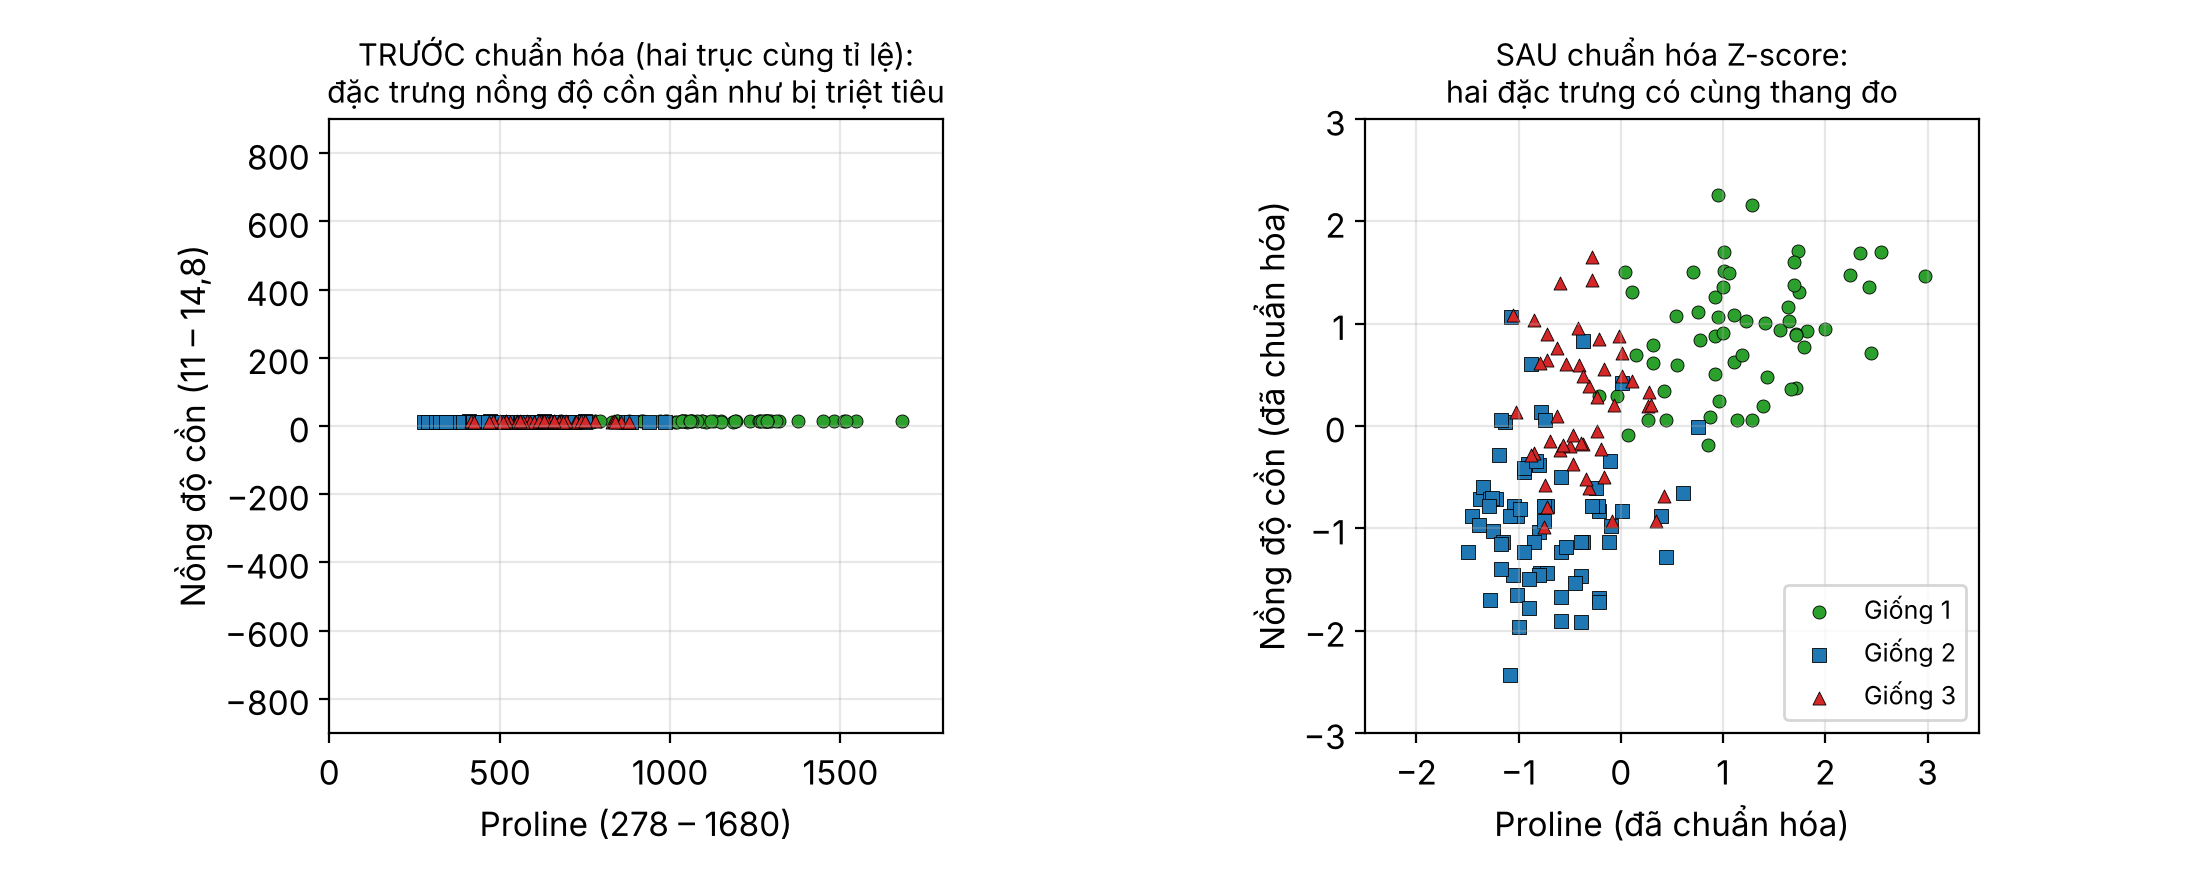
\includegraphics[width=0.9\linewidth]{h2_chuan_hoa.png}
\end{frame}

\begin{frame}{Bước 2 -- Tính khoảng cách}
\begin{columns}[c,totalwidth=\textwidth]
\begin{column}{0.47\textwidth}
{\footnotesize $d(Q,P) = \sqrt{(Q_1 - P_1)^2 + (Q_2 - P_2)^2}$}
\vspace{0.4em}

\small
\renewcommand{\arraystretch}{1.15}
\begin{tabular}{lll}
\rowcolor{bang}\textbf{Điểm} & \textbf{Phép tính} & \textbf{d}\\
A & $\sqrt{2^2+2^2}=\sqrt8$ & 2,83\\
B & $\sqrt{1^2+2^2}=\sqrt5$ & 2,24\\
C & $\sqrt{0^2+1{,}5^2}$ & 1,50\\
D & $\sqrt{1^2+0^2}=\sqrt1$ & \hl{1,00}\\
E & $\sqrt{2^2+2^2}=\sqrt8$ & 2,83\\
F & $\sqrt{3^2+1^2}=\sqrt{10}$ & 3,16\\
\end{tabular}

\vspace{0.3em}
Tính với \textbf{toàn bộ} $n$ điểm $\Rightarrow$ chi phí lớn nhất
\end{column}
\begin{column}{0.51\textwidth}
  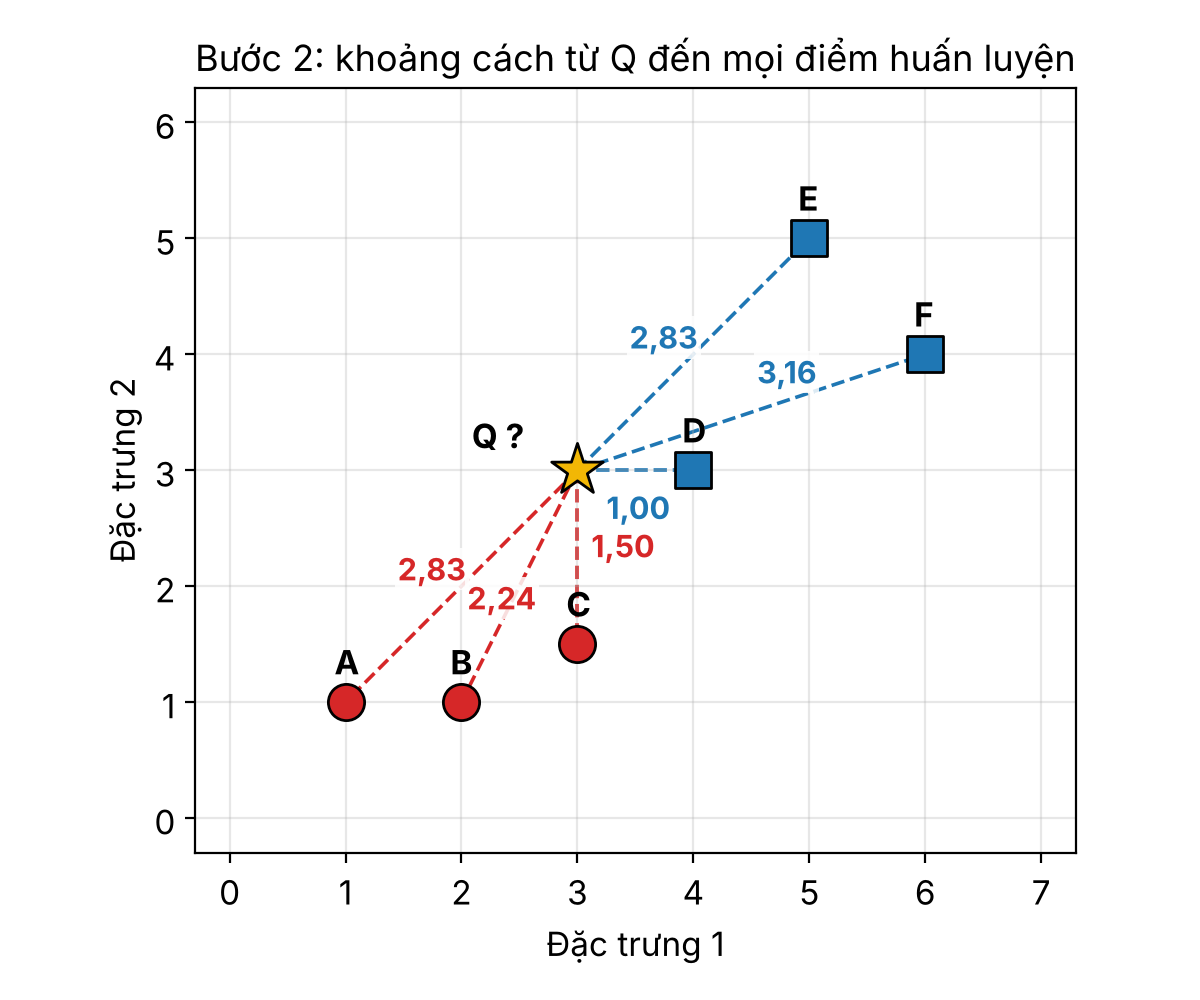
\includegraphics[width=\linewidth]{h3_do_khoang_cach.png}
\end{column}
\end{columns}
\end{frame}

\begin{frame}{Bước 3 -- Xác định K láng giềng}
\begin{itemize}
  \item Sắp xếp tăng dần: D (1,00) → C (1,50) → B (2,24) → A, E (2,83) → F (3,16)
  \item K = 3 $\Rightarrow$ $N_3(Q) = \{$\hl{D, C, B}$\}$
\end{itemize}
\vspace{0.2em}
\centering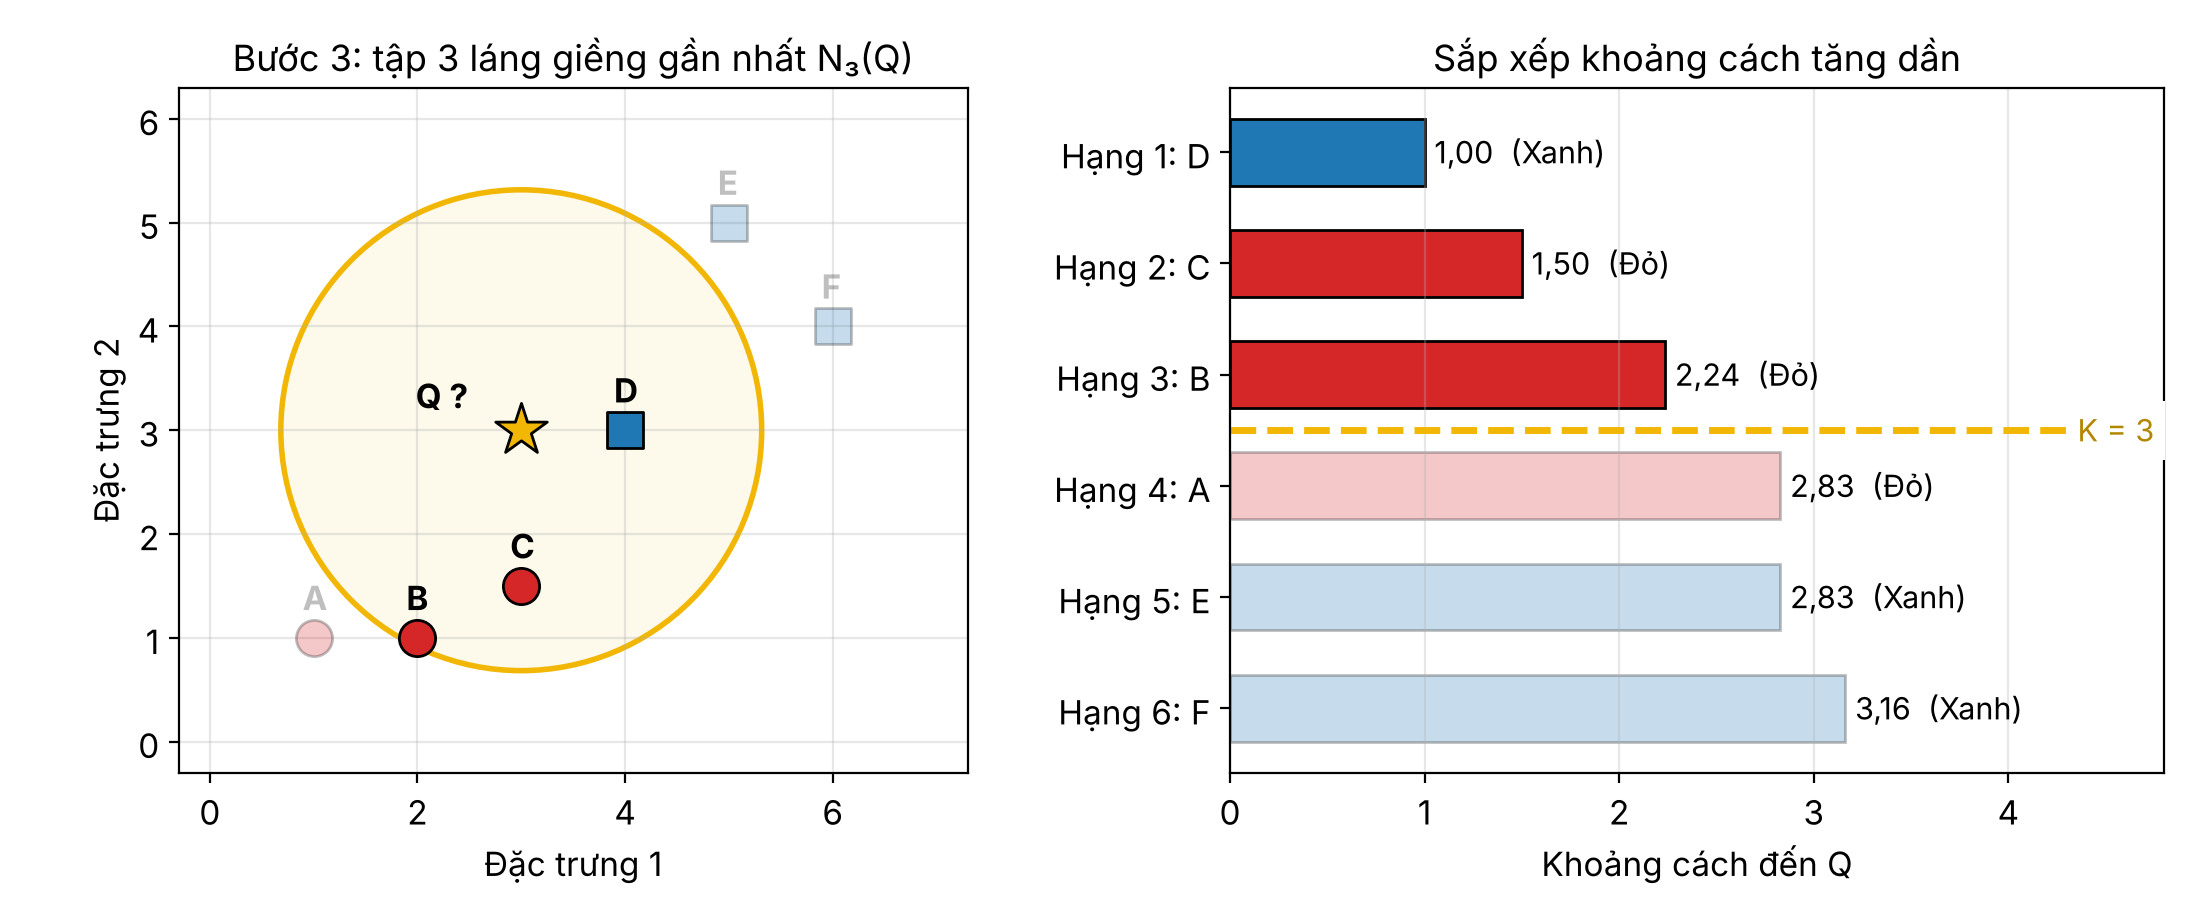
\includegraphics[width=0.96\linewidth]{h4_xep_hang.png}
\end{frame}

\begin{frame}{Bước 4 -- Biểu quyết đa số}
\begin{itemize}
  \item Lớp Đỏ: C, B -- \textbf{2 phiếu} \quad Lớp Xanh: D -- \textbf{1 phiếu} \quad $\Rightarrow$ \hl{$\hat y(Q)$ = Đỏ}
  \item Láng giềng gần nhất thuộc lớp Xanh, nhưng lớp Đỏ chiếm \textbf{đa số trong vùng lân cận}
\end{itemize}
\vspace{0.2em}
\centering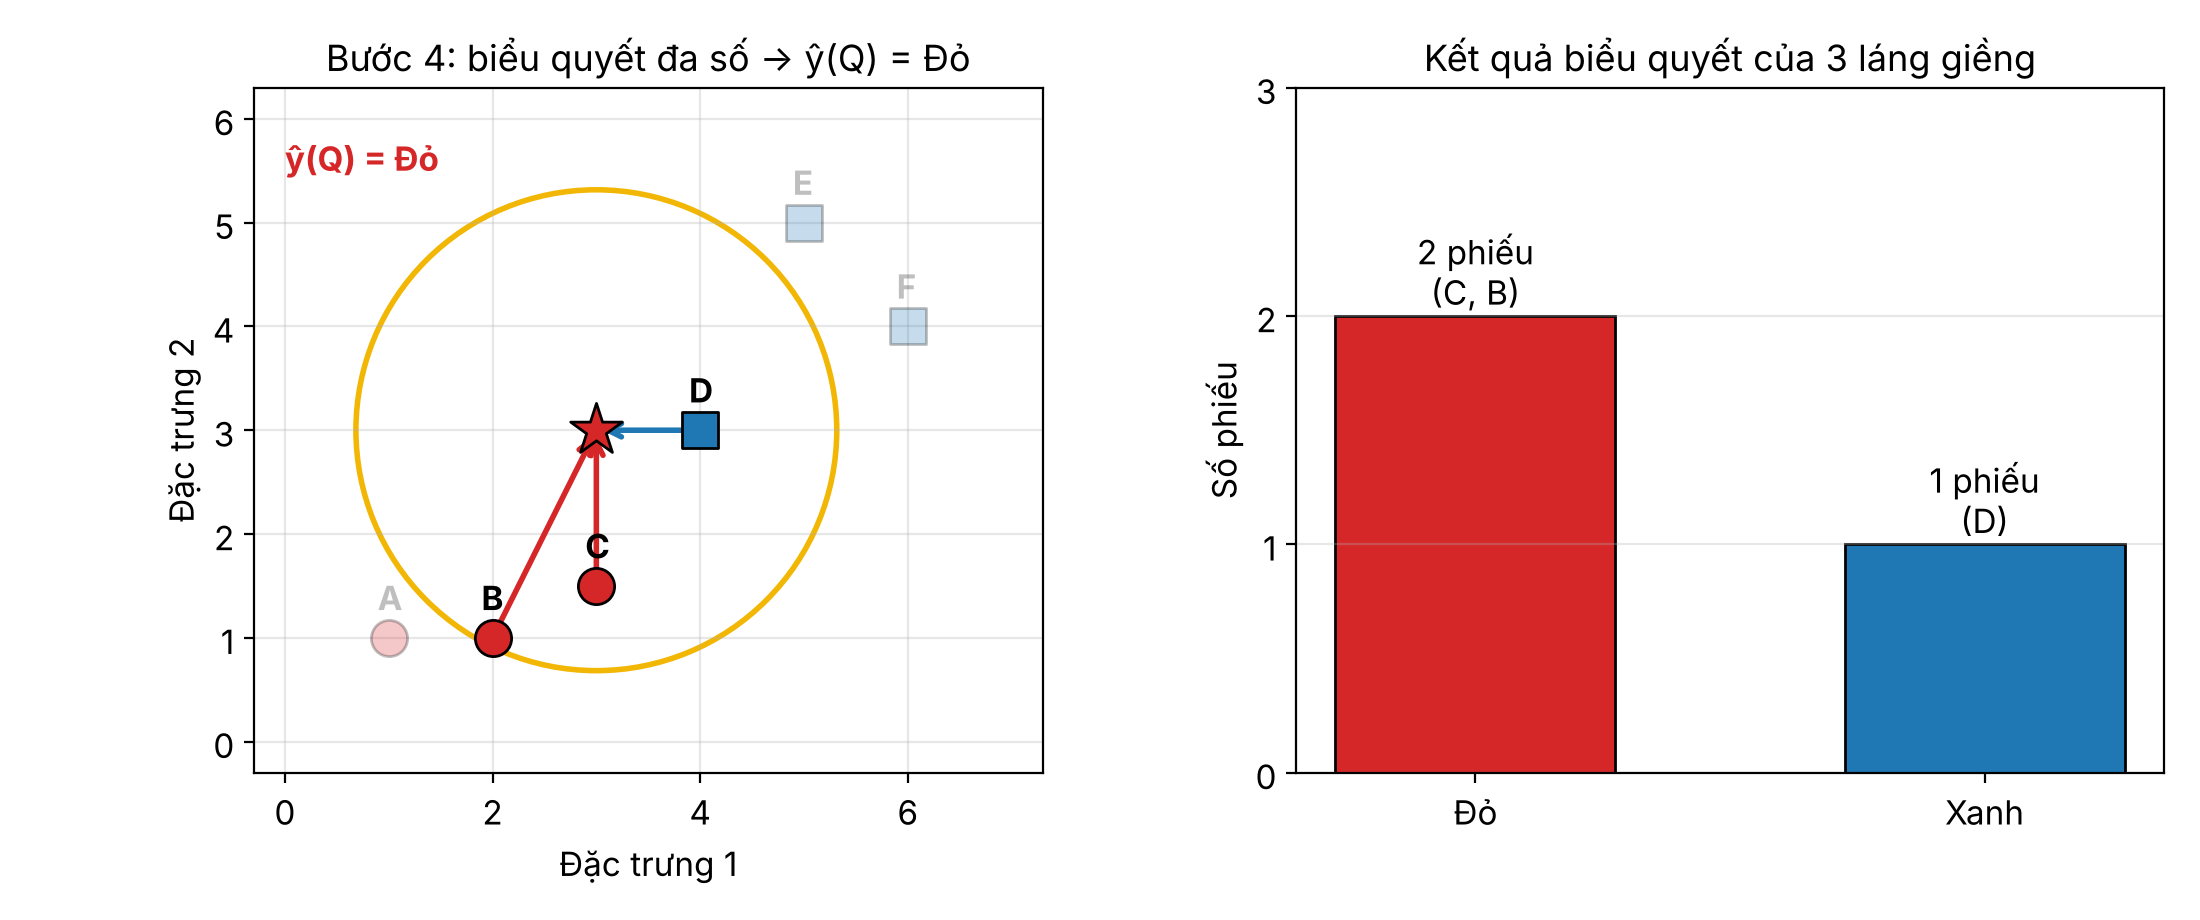
\includegraphics[width=0.96\linewidth]{h5_bo_phieu.png}
\end{frame}

\begin{frame}{Mã giả thuật toán KNN}
\begin{center}
\fcolorbox{chu}{white}{\parbox{0.97\linewidth}{\ttfamily\footnotesize\vspace{4pt}
\textbf{Input:} D \hspace{4em}// tập huấn luyện \{(x$_i$, y$_i$)\}\\
\hspace*{2.9em}x \hspace{4em}// điểm truy vấn\\
\hspace*{2.9em}K \hspace{4em}// số láng giềng\\
\textbf{Output:} ŷ \hspace{3.1em}// nhãn dự đoán\\[4pt]
L = $\emptyset$\\
\textbf{for each} (x$_i$, y$_i$) \textbf{in} D \textbf{do}\\
\hspace*{1.5em}L = L $\cup$ \{ (d(x, x$_i$), y$_i$) \} \hspace{1.5em}// Bước 2: tính khoảng cách\\
sắp xếp L tăng dần theo khoảng cách \hspace{0.5em}// Bước 3: xác định láng giềng\\
N = K phần tử đầu tiên của L\\
ŷ = nhãn xuất hiện nhiều nhất trong N \hspace{0.1em}// Bước 4: biểu quyết\\
\textbf{return} ŷ\vspace{4pt}}}
\end{center}
\end{frame}

\begin{frame}{Độ đo khoảng cách}
\vspace{0.3em}\small
\renewcommand{\arraystretch}{1.3}
\begin{tabularx}{\linewidth}{@{}l l X@{}}
\rowcolor{bang}\textbf{Độ đo} & \textbf{Công thức} & \textbf{Đặc điểm}\\
Euclid & $\sqrt{\sum_j (x_j - z_j)^2}$ & Độ dài đoạn thẳng -- \textbf{phổ biến nhất}\\
Manhattan & $\sum_j |x_j - z_j|$ & Tổng độ lệch tuyệt đối theo từng trục\\
Chebyshev & $\max_j |x_j - z_j|$ & Chỉ xét chiều có độ lệch lớn nhất\\
Cosine & $1 - \frac{x\cdot z}{\|x\|\,\|z\|}$ & Đo độ lệch về hướng, không phụ thuộc độ lớn\\
\end{tabularx}
\begin{itemize}
  \item Ví dụ $x=(1;2)$, $z=(4;6)$: Euclid = 5, Manhattan = 7, Chebyshev = 4
\end{itemize}
\centering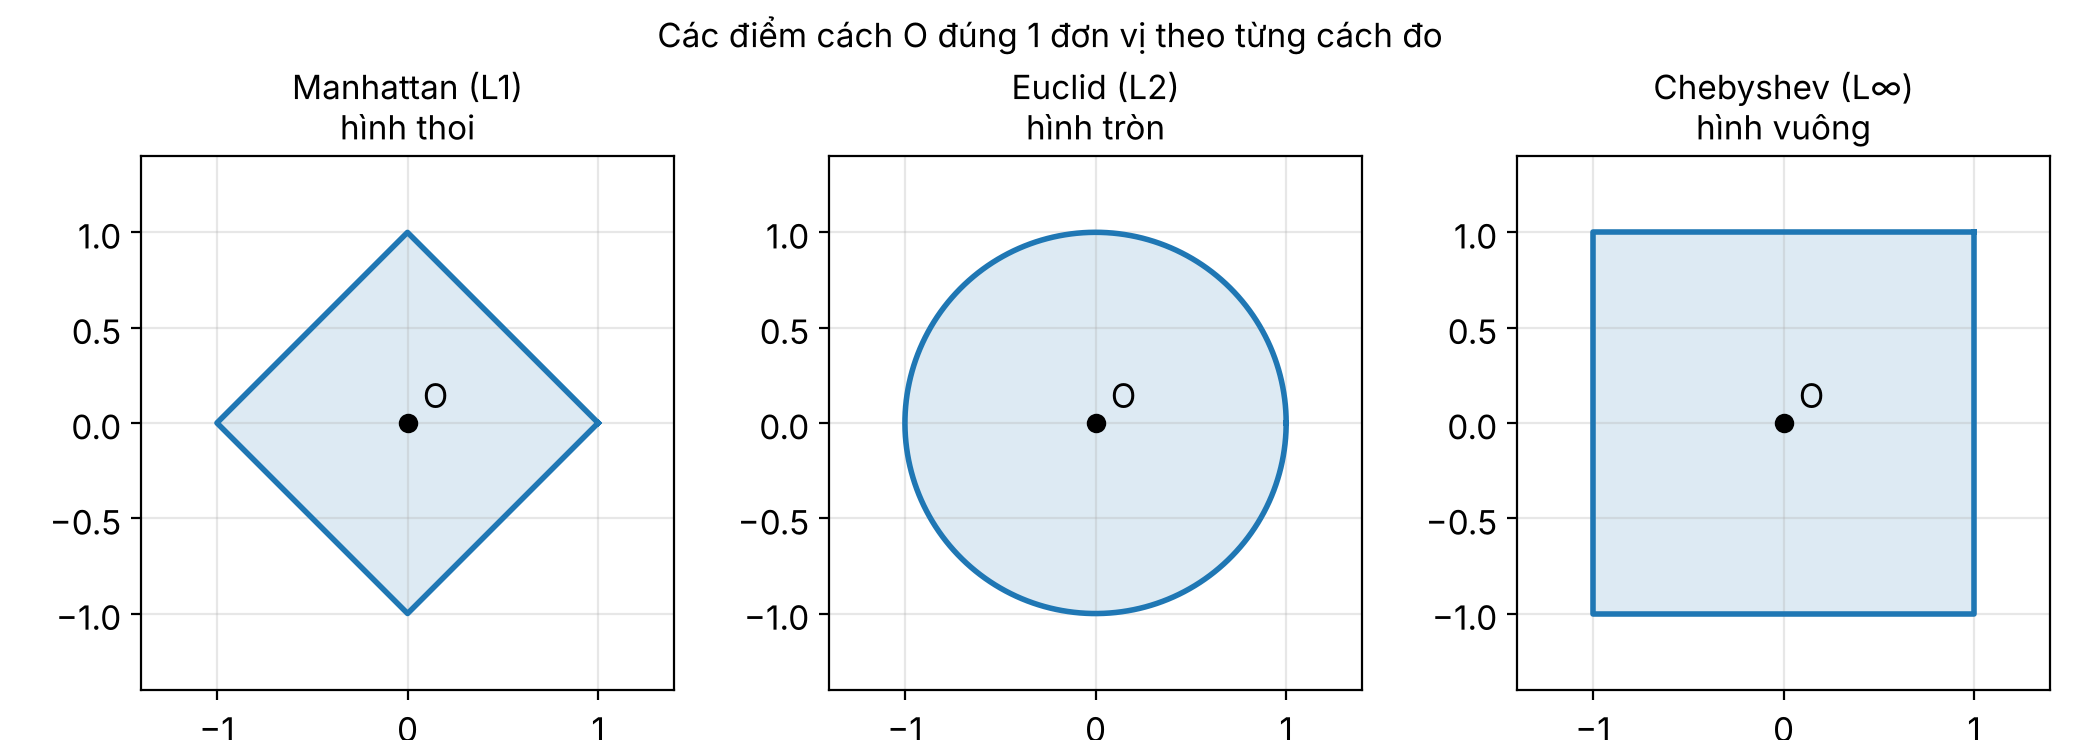
\includegraphics[width=0.68\linewidth]{h8_hinh_khoang_cach.png}
\end{frame}

\begin{frame}{Chuẩn hóa dữ liệu}
\begin{itemize}\setlength\itemsep{0.35em}
  \item Đặc trưng có \hl{miền giá trị lớn chi phối khoảng cách}: thu nhập (100 -- 1000) so với tuổi (18 -- 60)
\end{itemize}
\hop{Min-Max: $x' = \dfrac{x - \min}{\max - \min}$ \qquad Z-score: $x' = \dfrac{x - \mu}{\sigma}$ \quad ($\mu$: trung bình, $\sigma$: độ lệch chuẩn)}
\begin{itemize}\setlength\itemsep{0.35em}
  \item Ước lượng min, max, $\mu$, $\sigma$ \textbf{chỉ trên tập huấn luyện} (tránh rò rỉ dữ liệu)
  \item \textbf{Ví dụ} (tuổi; thu nhập triệu đồng): A = (25; 300) không mua, B = (44; 340) mua, Q = (43; 305)
  \begin{itemize}
    \item Không chuẩn hóa: $d(Q,A) \approx 18{,}7$, $d(Q,B) \approx 35{,}0$ $\Rightarrow$ \hl{không mua}
    \item Chuẩn hóa Min-Max: $d(Q,A) \approx 0{,}429$, $d(Q,B) \approx 0{,}046$ $\Rightarrow$ \hx{mua}
  \end{itemize}
  \item Chuẩn hóa làm \textbf{đảo ngược kết quả} vì tuổi của Q gần như trùng với B
\end{itemize}
\end{frame}

\begin{frame}{Lựa chọn tham số K}
\begin{columns}[c,totalwidth=\textwidth]
\begin{column}{0.55\textwidth}
\begin{itemize}\setlength\itemsep{0.5em}
  \item \textbf{K nhỏ} (K = 1):
  \begin{itemize}
    \item Phương sai cao, nhạy với nhiễu
    \item \hl{Quá khớp (overfitting)}
  \end{itemize}
  \item \textbf{K lớn}:
  \begin{itemize}
    \item Độ lệch cao, biên quyết định quá trơn
    \item \hl{Chưa khớp (underfitting)}
  \end{itemize}
  \item Lựa chọn K bằng \textbf{kiểm định chéo}
  \item Bài toán hai lớp: chọn \textbf{K lẻ} để tránh hòa phiếu
\end{itemize}
\end{column}
\begin{column}{0.43\textwidth}
  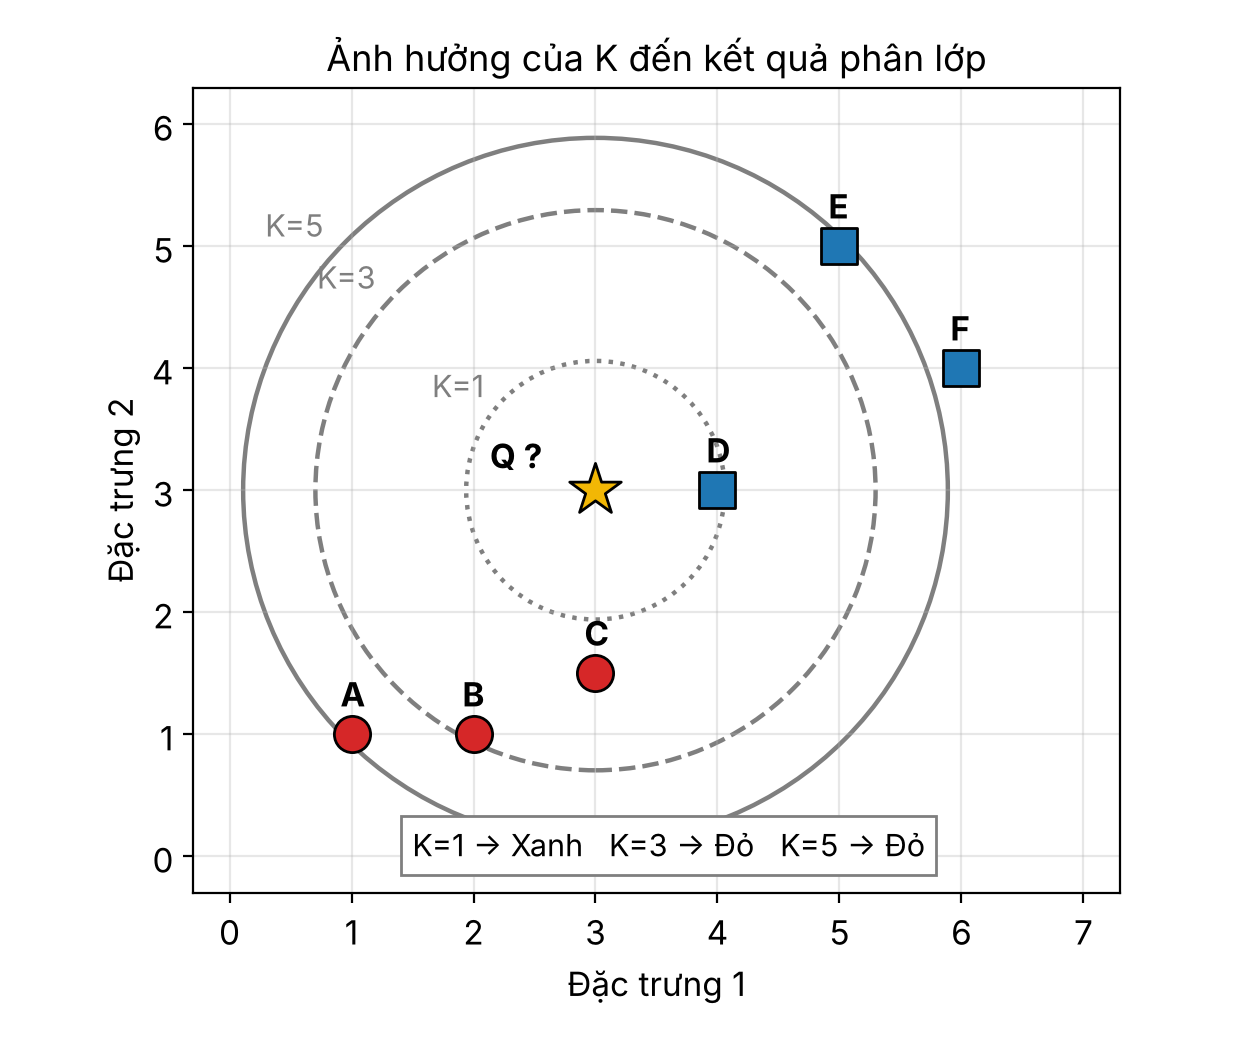
\includegraphics[width=\linewidth]{h6_anh_huong_k.png}
\end{column}
\end{columns}
\end{frame}

\begin{frame}{Kiểm định chéo: ví dụ}
\begin{itemize}\setlength\itemsep{0.4em}
  \item \textbf{Kiểm định chéo}: lần lượt dùng một phần dữ liệu làm tập đánh giá, phần còn lại làm dữ liệu tham chiếu, lấy trung bình độ chính xác
  \item Ví dụ: \textbf{Leave-One-Out} trên 6 điểm A--F
\end{itemize}
\vspace{0.2em}
\centering\small
\renewcommand{\arraystretch}{1.3}
\begin{tabular}{ccl}
\rowcolor{bang}\textbf{K} & \textbf{Độ chính xác} & \textbf{Giải thích}\\
1 & 5/6 & Phân lớp sai D do láng giềng gần nhất là C (Đỏ)\\
\hl{3} & \hl{6/6} & Cao nhất $\Rightarrow$ \hl{chọn K = 3}\\
5 & 0/6 & Tập láng giềng là toàn bộ dữ liệu còn lại (chưa khớp)\\
\end{tabular}
\end{frame}

\begin{frame}{KNN có trọng số, hồi quy}
\begin{itemize}\setlength\itemsep{0.45em}
  \item \textbf{KNN có trọng số} (Dudani, 1976): trọng số \hl{tỉ lệ nghịch với khoảng cách}
\end{itemize}
\hop{$w_i = \dfrac{1}{d(x, x_i)}$ \qquad lớp thắng = lớp có \textbf{tổng} $w$ lớn nhất}
\begin{itemize}\setlength\itemsep{0.45em}
  \item Ví dụ Q: Xanh = 1/1 = 1,00; Đỏ = 1/1,5 + 1/2,24 = 1,12 $\Rightarrow$ vẫn \hl{Đỏ}. Giảm phụ thuộc vào K, hạn chế hòa phiếu
  \item \textbf{KNN hồi quy}: dự đoán giá trị liên tục bằng \textbf{trung bình} của K láng giềng
  \begin{itemize}
    \item Giá nhà 72 m², K = 3: nhà 60, 70, 80 m² giá 1,8; 2,1; 2,6 tỷ
    \item $\hat y = (1{,}8 + 2{,}1 + 2{,}6)/3 \approx 2{,}17$ tỷ
  \end{itemize}
\end{itemize}
\end{frame}

\begin{frame}{Một số vấn đề mở rộng}
\begin{itemize}\setlength\itemsep{0.7em}
  \item \textbf{Tốc độ}
  \begin{itemize}
    \item Huấn luyện $O(1)$; mỗi lần dự đoán có chi phí $O(n \cdot d)$
    \item Tăng tốc: KD-Tree, tìm láng giềng gần xấp xỉ
  \end{itemize}
  \item \textbf{Cơ sở lý thuyết} (Cover \& Hart, 1967)
  \begin{itemize}
    \item Khi $n \to \infty$: sai số của 1-NN $\le$ \hl{2 lần} sai số Bayes
  \end{itemize}
  \item \textbf{Lời nguyền số chiều}
  \begin{itemize}
    \item Số chiều lớn $\Rightarrow$ khoảng cách giữa các cặp điểm xấp xỉ nhau
    \item Cần giảm chiều dữ liệu (ví dụ PCA)
  \end{itemize}
\end{itemize}
\end{frame}

% =====================================================================
% 4. THỰC NGHIỆM
% =====================================================================
\mucluc{4}

\begin{frame}{Dữ liệu Iris}
\begin{columns}[c,totalwidth=\textwidth]
\begin{column}{0.44\textwidth}
\begin{itemize}\setlength\itemsep{0.45em}
  \item Bộ dữ liệu kinh điển (Fisher, 1936), có sẵn trong scikit-learn
  \item \hx{150} bông hoa, \hx{3} loài, mỗi loài 50 bông
  \item Sử dụng \hx{2} đặc trưng: chiều dài và chiều rộng \textbf{cánh hoa} (cm)
  \item Setosa \textbf{tách biệt}; Versicolor và Virginica \textbf{chồng lấn một phần}
  \item Cùng đơn vị cm $\Rightarrow$ \textbf{không cần chuẩn hóa}
\end{itemize}
\end{column}
\begin{column}{0.54\textwidth}
  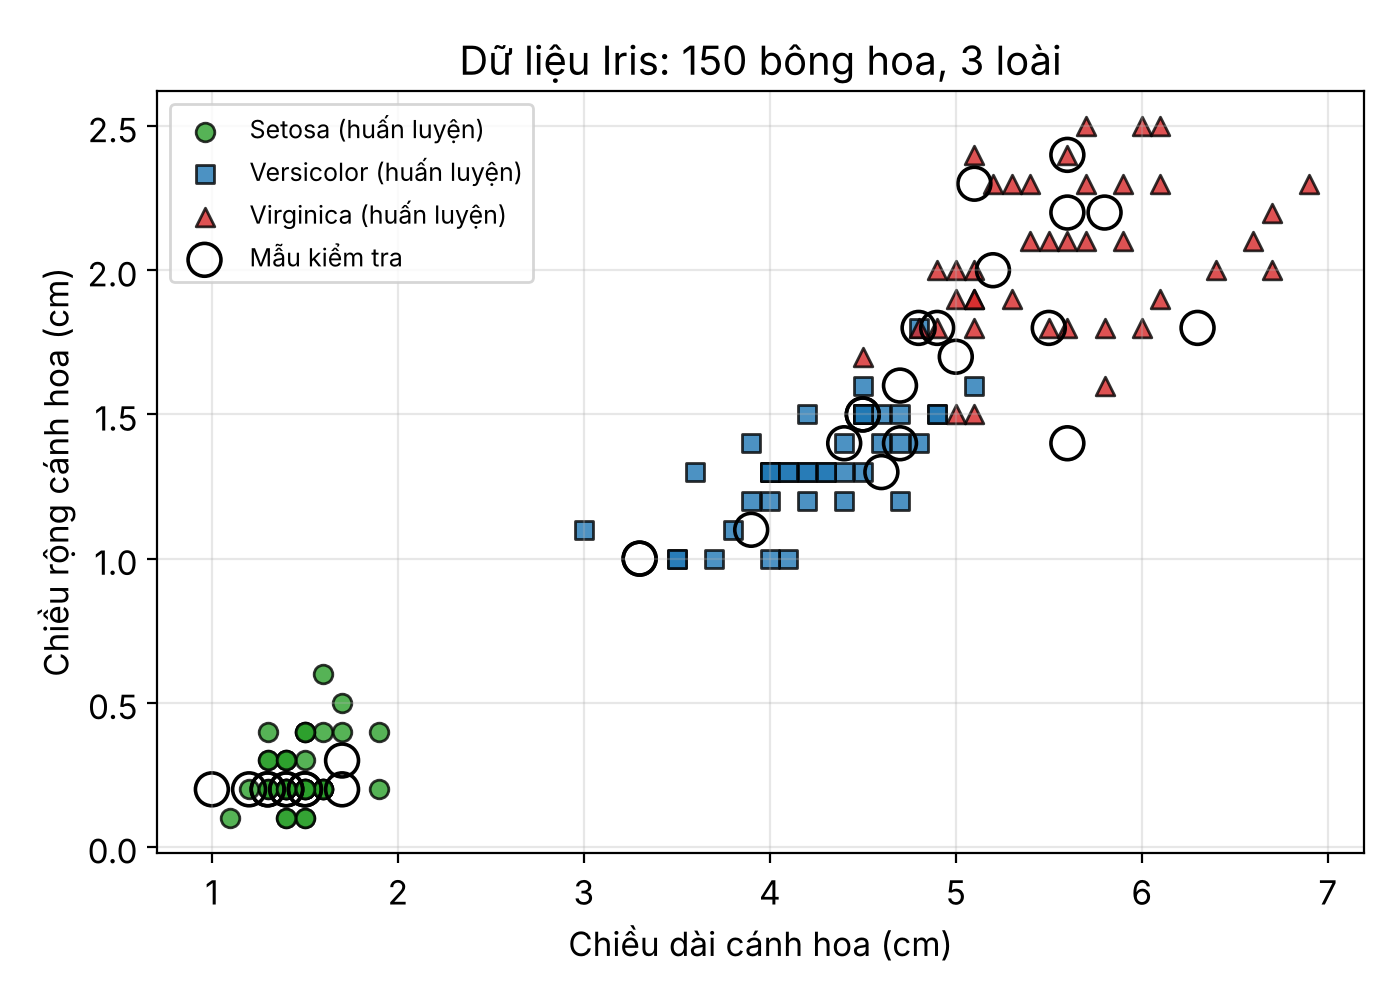
\includegraphics[width=\linewidth]{tn_du_lieu.png}
\end{column}
\end{columns}
\end{frame}

\begin{frame}{Phương pháp và cài đặt}
\begin{enumerate}\setlength\itemsep{0.25em}
  \item Tập huấn luyện 80\% (120 mẫu), tập kiểm tra 20\% (30 mẫu), phân tầng theo loài
  \item Lựa chọn K bằng \textbf{kiểm định chéo 10-fold} trên tập huấn luyện
  \item Phân lớp 30 mẫu kiểm tra bằng KNN tự cài đặt
  \item Đánh giá: \textbf{độ chính xác} và \textbf{ma trận nhầm lẫn}
\end{enumerate}
\vspace{0.3em}
\colorbox{bang}{\parbox{0.98\linewidth}{\ttfamily\footnotesize\vspace{3pt}%
def knn\_predict(X\_train, y\_train, x, k):\\
\hspace*{1em}d = np.sqrt(((X\_train - x)**2).sum(axis=1)) \hspace{1em}\textcolor{gray}{\# Bước 2}\\
\hspace*{1em}idx = np.argsort(d)[:k] \hspace{9.6em}\textcolor{gray}{\# Bước 3}\\
\hspace*{1em}return Counter(y\_train[idx]).most\_common(1)[0][0] \textcolor{gray}{\# Bước 4}\vspace{3pt}}}
\begin{itemize}
  \item Kiểm chứng: trùng khớp \hl{30/30} dự đoán với KNeighborsClassifier (scikit-learn)
\end{itemize}
\end{frame}

\begin{frame}{Lựa chọn tham số K}
\begin{columns}[c,totalwidth=\textwidth]
\begin{column}{0.6\textwidth}
  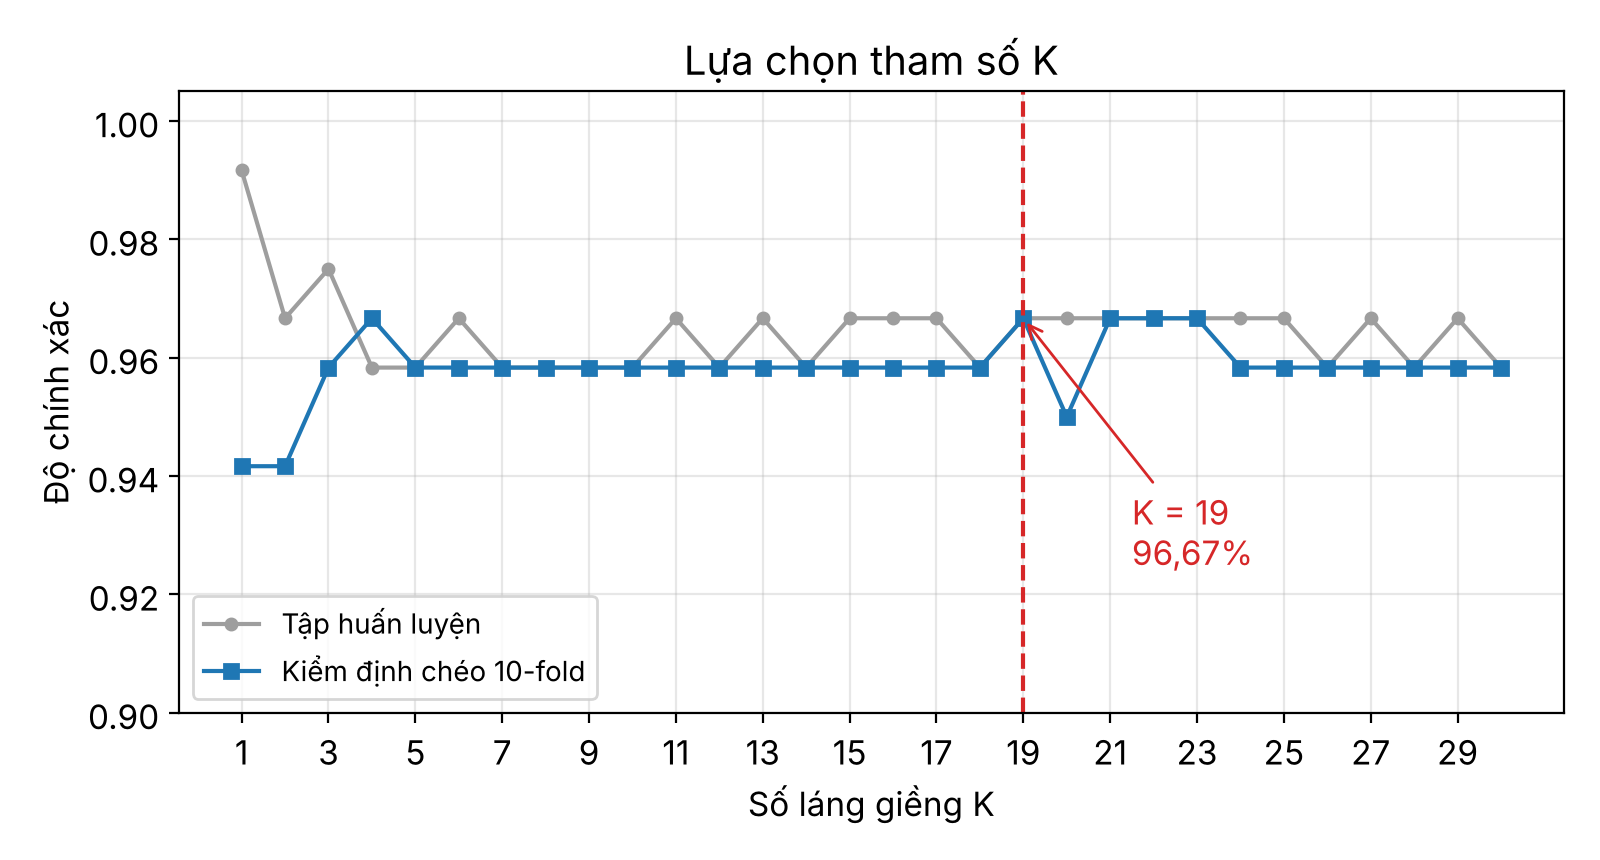
\includegraphics[width=\linewidth]{tn_chon_k.png}
\end{column}
\begin{column}{0.38\textwidth}
\begin{itemize}\setlength\itemsep{0.5em}\small
  \item \textbf{K = 1}: 99,17\% trên tập huấn luyện, 94,17\% kiểm định chéo $\Rightarrow$ \hl{quá khớp}
  \item K tăng: độ chính xác ổn định quanh 95,8\% -- 96,7\%
  \item Lớp tách biệt tốt $\Rightarrow$ ít nhạy với K
  \item Lựa chọn \hx{K = 19} (96,67\%)
\end{itemize}
\end{column}
\end{columns}
\end{frame}

\begin{frame}{Kết quả trên tập kiểm tra}
\begin{columns}[c,totalwidth=\textwidth]
\begin{column}{0.46\textwidth}
  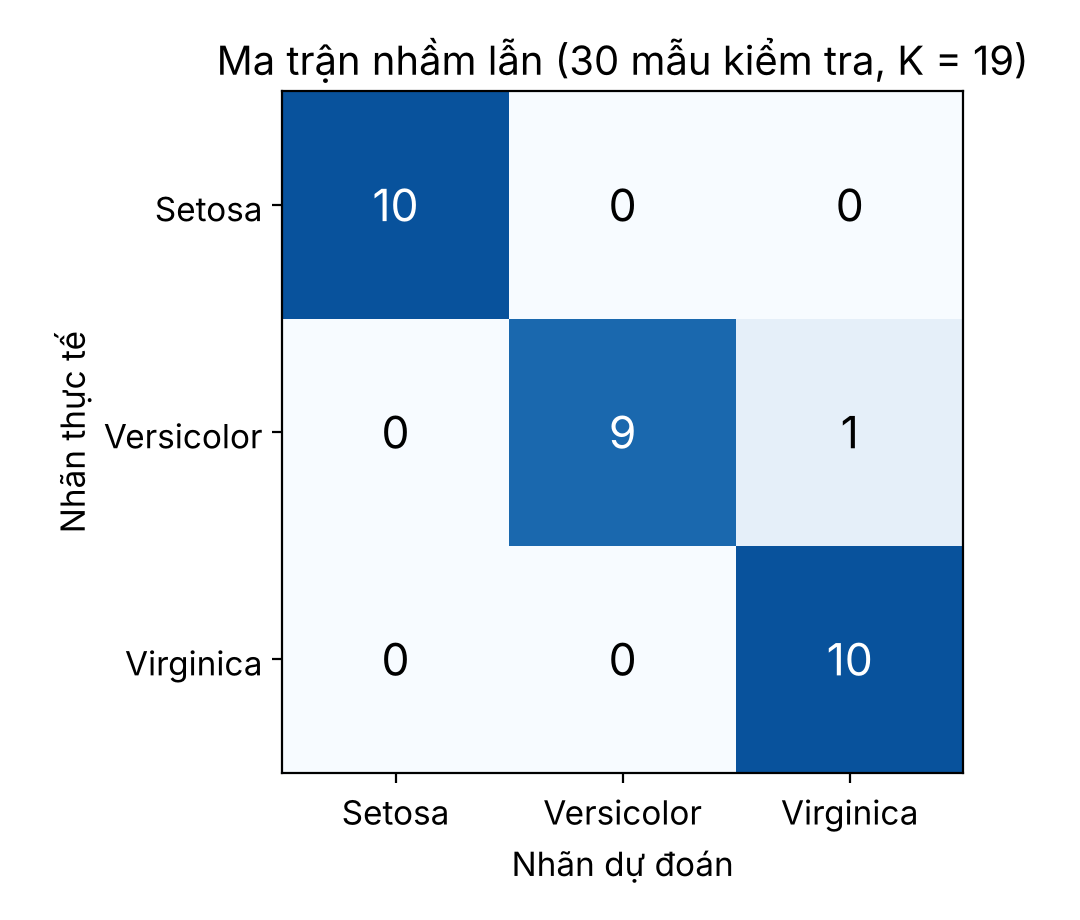
\includegraphics[width=\linewidth]{tn_ma_tran.png}
\end{column}
\begin{column}{0.52\textwidth}
\begin{itemize}\setlength\itemsep{0.55em}
  \item Phân lớp đúng \hx{29/30} bông hoa
  \item Accuracy = \hx{96,67\%}
  \item Setosa: 10/10, Virginica: 10/10
  \item Versicolor: 9/10 -- \hl{1 bông bị nhầm thành Virginica}
\end{itemize}
\end{column}
\end{columns}
\end{frame}

\begin{frame}{Vùng phân lớp và phân tích sai số}
\begin{columns}[c,totalwidth=\textwidth]
\begin{column}{0.56\textwidth}
  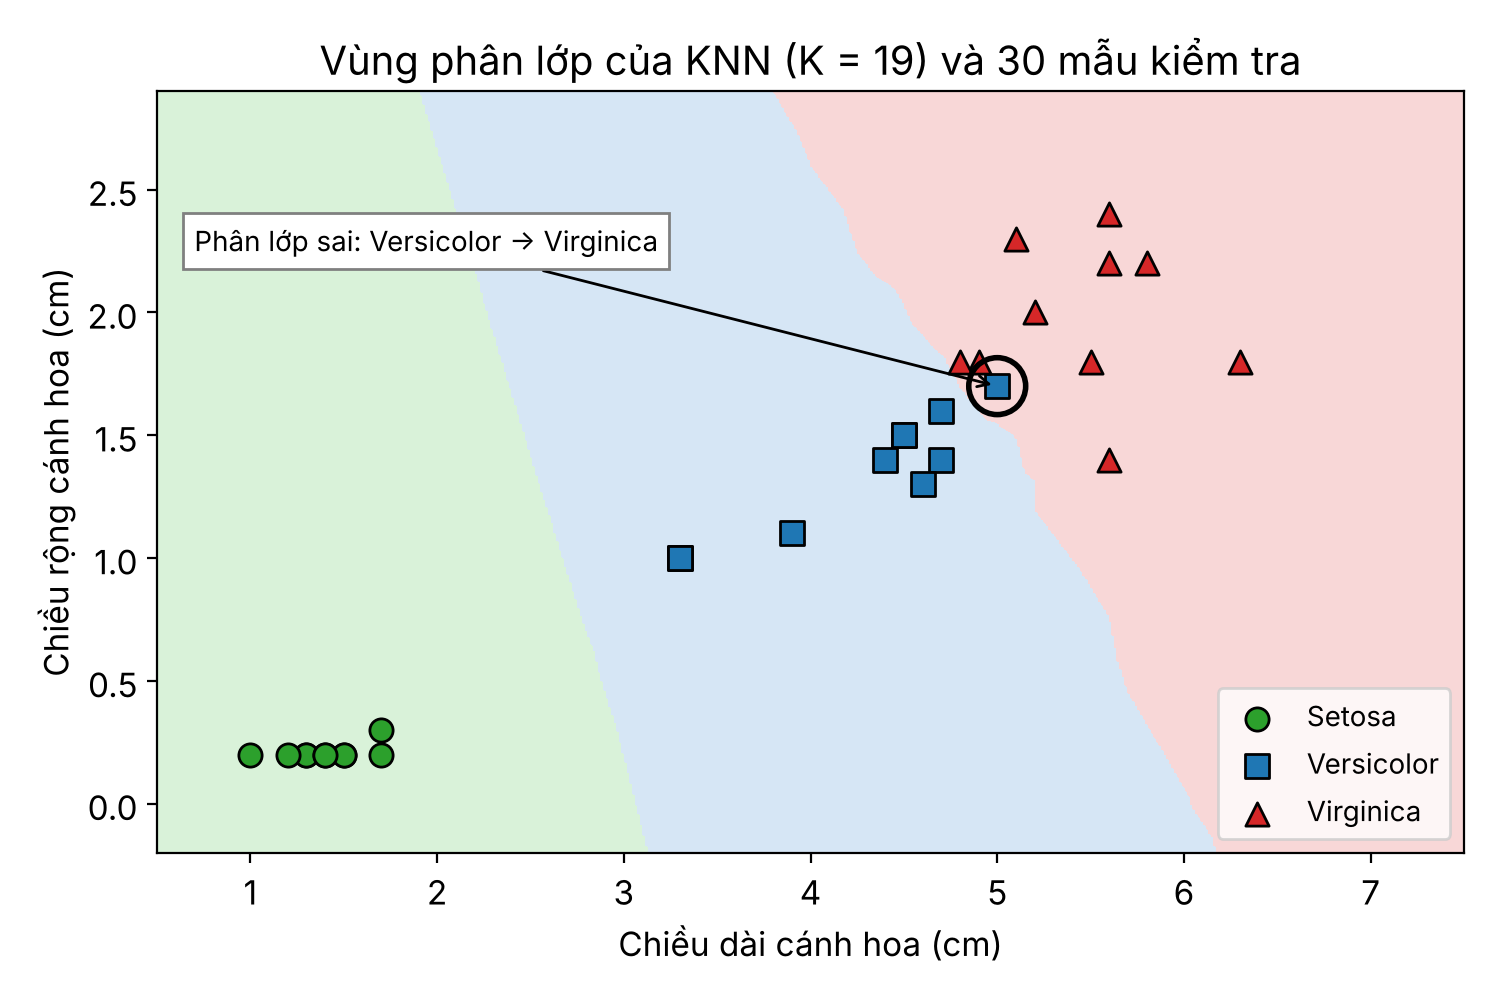
\includegraphics[width=\linewidth]{tn_vung_phan_lop.png}
\end{column}
\begin{column}{0.42\textwidth}
\begin{itemize}\setlength\itemsep{0.5em}\small
  \item Mẫu sai: cánh hoa 5,0 cm $\times$ 1,7 cm, nằm tại \textbf{vùng chồng lấn} Versicolor -- Virginica
  \item 19 láng giềng: \hl{12 Virginica}, 7 Versicolor $\Rightarrow$ biểu quyết ra Virginica
  \item Mẫu có số đo giống loài khác hơn loài của chính nó -- giới hạn của dữ liệu, không phải lỗi cài đặt
\end{itemize}
\end{column}
\end{columns}
\end{frame}

\begin{frame}{Tổng hợp kết quả}
\centering\small
\renewcommand{\arraystretch}{1.6}
\begin{tabular}{ll}
\rowcolor{bang}\textbf{Nội dung} & \textbf{Kết quả}\\
Tham số K & K = 19 (kiểm định chéo 96,67\%)\\
Độ chính xác trên tập kiểm tra & \hx{96,67\%} (29/30 mẫu)\\
Mẫu phân lớp sai & 1 Versicolor $\to$ Virginica (vùng chồng lấn)\\
Kiểm chứng cài đặt & Trùng khớp 30/30 với scikit-learn\\
\end{tabular}
\vspace{0.6em}
\begin{itemize}
  \item KNN đạt độ chính xác cao với thuật toán đơn giản, không cần huấn luyện
  \item Sai số chỉ xuất hiện tại vùng chồng lấn giữa hai lớp
\end{itemize}
\end{frame}

\mucluc{5}

\begin{frame}{Kết luận}
\begin{itemize}\setlength\itemsep{0.45em}
  \item \textbf{KNN}: phân lớp phi tham số dựa trên \hl{tương đồng cục bộ} và \hl{biểu quyết đa số}
  \item Phân loại hoa Iris: K = 19 $\Rightarrow$ Accuracy \hx{96,67\%} (29/30 mẫu)
  \item \textbf{Điểm mạnh}
  \begin{itemize}
    \item Đơn giản, có khả năng diễn giải
    \item Không cần huấn luyện; biểu diễn được biên quyết định phi tuyến
    \item Dùng được cho phân lớp và hồi quy
  \end{itemize}
  \item \textbf{Điểm yếu}
  \begin{itemize}
    \item Chi phí dự đoán $O(n\cdot d)$ lớn khi dữ liệu lớn
    \item Nhạy với thang đo, nhiễu; chịu ảnh hưởng của lời nguyền số chiều
    \item Cần lựa chọn K; thiên về lớp đa số khi dữ liệu mất cân bằng
  \end{itemize}
\end{itemize}
\end{frame}

\begin{frame}{Tài liệu tham khảo}
\footnotesize
\begin{itemize}\setlength\itemsep{0.35em}
  \item Cover, T., Hart, P. (1967). Nearest neighbor pattern classification. \textit{IEEE Trans. Information Theory}.
  \item Dudani, S. A. (1976). The distance-weighted k-nearest-neighbor rule. \textit{IEEE Trans. SMC}.
  \item Wu, X. et al. (2008). Top 10 algorithms in data mining. \textit{Knowledge and Information Systems}.
  \item Fisher, R. A. (1936). The use of multiple measurements in taxonomic problems. \textit{Annals of Eugenics}.
  \item Pedregosa, F. et al. (2011). Scikit-learn: Machine Learning in Python. \textit{JMLR}.
  \item Han, J., Kamber, M., Pei, J. (2011). \textit{Data Mining: Concepts and Techniques}. Morgan Kaufmann.
  \item Trịnh Thành. \textit{Bài giảng Khai phá dữ liệu}. Trường CNTT Phenikaa.
\end{itemize}
\end{frame}

\begin{frame}[plain]
  \vspace*{2.2cm}
  \begin{flushright}
    {\titlefont\color{tieude}\fontsize{30}{36}\selectfont Cảm ơn thầy/cô\par và các bạn!\par}
    \vspace{0.4cm}
    {\large\color{gray} Hỏi -- Đáp\par}
  \end{flushright}
\end{frame}

\end{document}
